\documentclass{llncs}
\usepackage{epsf}
\usepackage{graphicx}
\usepackage[utf8]{inputenc}

\begin{document}

\title{Predictive Text Entry of Agglutinative Languages using Morphological Segmentation and Phonological Restrictions}

\author{\ldots\\\ldots\\\ldots}
\institute{\ldots}

\maketitle

\begin{abstract}
Systems for predictive text entry on ambiguous keyboards typically
rely on dictionaries with word frequencies which are used to suggest
the most likely words matching user input. This approach is
insufficient for agglutinative languages, where morphological
phenomena increase the rate of out-of-vocabulary words. We propose a
method for text entry, which circumvents the problem of
out-of-vocabulary words, by replacing the dictionary with a Markov
chain on morph sequences combined with a third order hidden Markov
model (HMM) mapping key sequences to letter sequences and phonological
constraints for pruning suggestion lists. We evaluate our method by
constructing text entry systems for Finnish and Turkish and comparing
our systems with published text entry systems and the text entry systems
of three commercially available mobile phones. Measured using the
keystrokes per character ratio (KPC) \cite{MacKenzie02kspc}, we
achieve superior results. For training, we use corpora, which are
segmented using unsupervised morphological segmentation.
\end{abstract}

\section{Introduction}

Mobile phone text messages are a hugely popular means of
communication, but mobile phones are not especially well-suited for
inputting text because of their small size and often limited
keyboard. There exist several technological solutions for text entry
on mobile phones and other limited keyboard devices. This paper is
concerned with a technology called \textit{predictive text entry}, which
utilizes redundancy in natural language in order to enable efficient
text entry using limited keyboards (typically having 12 keys).

The subject of predictive text entry has been extensively studied, but
the studies have mainly concentrated on predictive text entry of
English. Because of the limited morphological complexity of English,
these approaches have usually been able to rely on an extensive
dictionary along with word frequencies, since a sufficiently large
English dictionary almost eliminates the problem of out-of-vocabulary
(OOV) words. E.g. \cite{klarlund/2002} reports low OOV word rates of
1.42 \% for a training set containing the $40,000$ most frequent words
in the North American Business News Corpus and a test set consisting
of $54,265$ sentences from the same corpus.

For morphologically complex languages like Finnish and Turkish,
productive inflection, derivation and compounding raise the number of
out-of-vocabulary words regardless of the size of the dictionary,
i.e. the vocabulary growth rate does not
converge~\cite{Creutz_morph-basedspeech}, which means that
out-of-vocabulary words present a serious problem for dictionary based
approaches to predictive text entry.

In this paper we present an approach to predictive text entry which is
based upon a morphologically segmented training corpus, which is used
to construct a probabilistic model of morphotax. We additionally use a
probabilistic model on letter sequences and phonological constraints,
which limit the results of the probabilistic models. We show that this
model delivers superior results compared to an existing dictionary
based model~\cite{silfverberg/2011/cla} for text entry of Finnish when
evaluated on actual text-message data using the keystroke per
character ratio (KPC)~\cite{MacKenzie02kspc}. We also compare our
method to the predictive text entry in three commercially available
mobile phones and show that our approach gives superior KPC.

Apart from phonological rules, our approach is entirely unsupervised
and data-driven, since we use the unsupervised morphological
segmentation system Morfessor \cite{Creutz07ACMTSLP} for segmenting
the training corpus and the tools for constructing POS-taggers from
the HFST interface~\cite{hfst/2011}. We show that our method can also
be applied to another agglutinative language besides Finnish, namely
Turkish. We compare the Turkish text entry system with an existing
text entry system, which is based on a Markov model on letter
sequences and show that our approach gives a substantial improvement
in KPC.

The paper is structured as follows. In section~\ref{earlier-work} we
present some earlier approaches to predictive text entry. In
section~\ref{model}, we present the components of our model for text
entry and explain how these models are combined into a system for
predictive text entry.  In Section~\ref{data} we describe the
training and test corpora used in constructing and testing predictive
text entry systems for Finnish and Turkish together with the
phonological rules which are used to realize Finnish vowel
harmony. Evaluation of the systems is presented in
section~\ref{evaluation} and the results are discussed in
section~\ref{discussion}. Finally we present some concluding remarks
and future work directions in section~\ref{conclusion}.

\section{Related Approaches to Text Entry}\label{earlier-work}

The mobile phone keypad is a so called clustered keyboard, where each
key can be used to enter several letters. E.g. on the Finnish mobile
phone keypad in Figure~\ref{keypad} the key 2 is used to enter the
letters "a", "b", "c", "\"{a}" and "å".

The original method for text entry is the so called
\textit{multitap-method}. When entering text in multitap mode, each key is
pressed multiple times to scroll through the list of letters that are
associated with the key. As text-messages have gained popularity, other
faster methods for text entry have been devised. These can broadly be
classified into movement minimization techniques, which concentrate on
keypad layout and language prediction techniques, which use linguistic
models to disambiguate ambiguous user input~\cite{Mackenzie/HCI/2002}.

The most widely used language prediction techniques are dictionary
based techniques, which disambiguate suggestions based on word
frequencies. The best known example of a dictionary based system is
the commercially successful T9-system~\cite{t9-patent}. There are many
variants of dictionary based methods. E.g. some methods try to guess
the word before all characters have been typed. Some approaches also
include information on the probability of word
sequences~\cite{Mackenzie/HCI/2002}.

\begin{figure}[hbt!]
\begin{center}
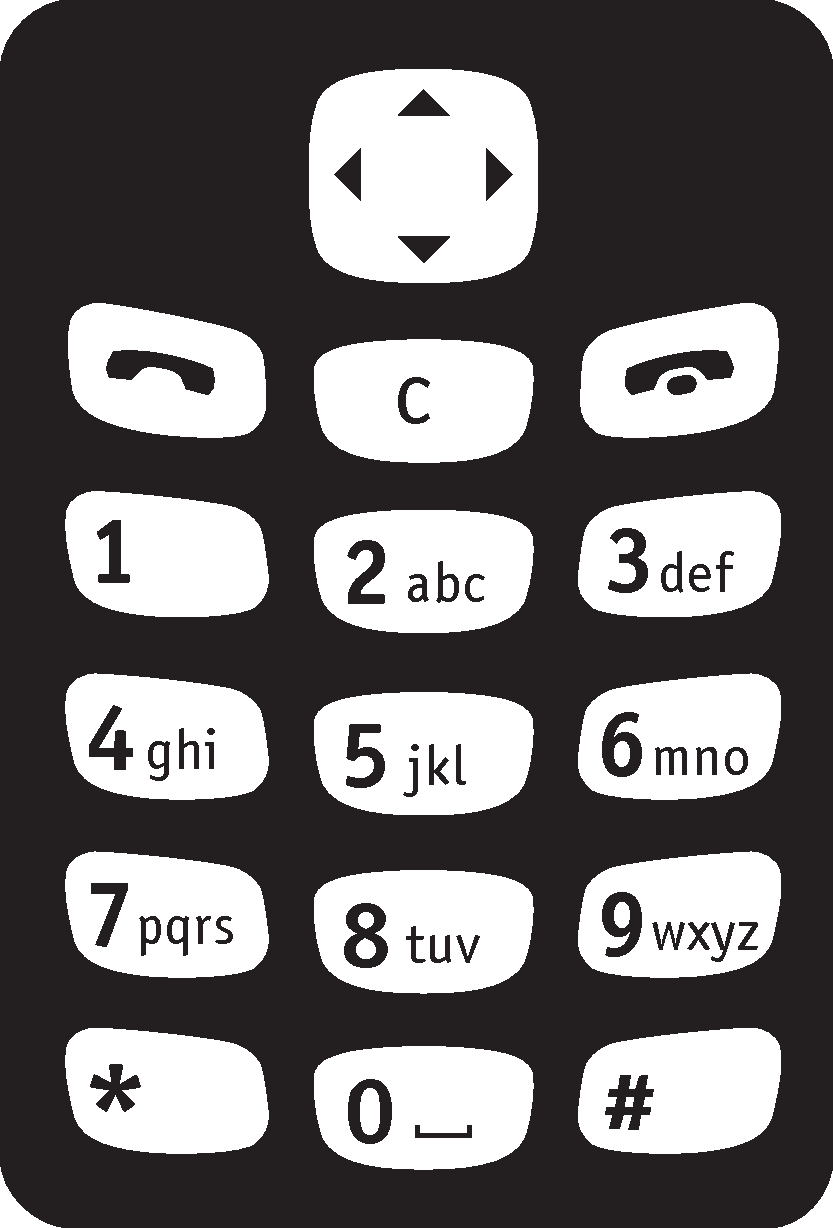
\includegraphics[width=1.1in]{Nappaimet.pdf}
\caption{The 12-key keypad of a typical Finnish mobile phone. There
  are three letters in the Finnish alphabet "\"{a}", "å" and "\"{o}",
  which are not shown on the keypad. The letters "\"{a}" and "å" are
  entered pressing key "2" four times and five times respectively. The
  letter "\"{o}" is entered by pressing the key "6" four
  times.}\label{keypad}
\end{center}
\end{figure}

As we noted in the introduction, dictionary based methods are not
optimal for agglutinative languages, where the OOV rate remains high
even with large dictionaries. Two published approaches suitable for
agglutinative languages are known to the authors: prefix-based
disambiguation~\cite{Mackenzie01letterwise:prefix-based} and
disambiguation of output using a probabilistic model on letter
sequences~\cite{Tantug:2010}. The methods resemble each other. Both
methods use the previous letter context to guess the next letter, but
in the prefix-based approach, an incorrectly guessed letter is
corrected immediately after it has been entered. When using a
probabilistic model on letter sequences, the user first inputs all
letters in the word and then scrolls through a list of suggestion
words matching the input.

Our own method utilizes a similar probabilistic model on letter
sequences as~\cite{Tantug:2010}, though we use a hidden Markov
model. The novel aspects of our method are (1) utilizing a
morphologically segmented training corpus in order to construct a
probabilistic model of words as morph sequences and (2) using
phonological constraints for filtering impossible suggestions. To the
best of our knowledge, this has not been tried before in the domain of
text-entry. In the related domain of speech recognition, similar
approaches have yielded good results~\cite{Creutz_morph-basedspeech}
for agglutinative languages.

\section{A Probabilistic Model of Word Structure}\label{model}

Predictive text entry can be seen as a labeling task, where every key
in a sequence of keys is assigned its most likely letter. The usual
approach to such tasks are stochastic model with hidden variables,
such as an HMM.

Though predictive text entry can be implemented fairly well using
n-gram models (such as HMMs) on letter sequences, as exemplified
by~\cite{Tantug:2010}, there are problems with this approach. An HMM
cannot encode very long dependencies inside words, which leads to
difficulties since it is not possible to adequately separate stems
from affixes or to handle long phonological dependencies like vowel
harmony. Higher order HMMs are not useful in practice because of
efficiency problems~\cite{Tantug:2010}.

In order to construct a general prediction model, which still
represents word structure at a higher level than at the level of
single letters, we represent words as morph sequences, which are
extracted from an automatically segmented training corpus.

To illustrate the usefulness of our approach we look at some Finnish
word forms. Consider the word form "taloa" (sg. partitive case of
the word house). Automatic segmentation of the training corpus might
give the segmentation "talo+a", into the stem "talo" and the ending
"a". If the word form "taloakin" (sg. partitive case of "talo" with
the clitic "kin") does not occur in the training data, we can still
estimate its probability by utilizing the frequencies of the morph
combinations "talo + a" and "a + kin",

Our model for word structure is a Markov chain of morph
sequences. Data sparseness is likely to be a serious problem, since
there are tens of thousands of morphs, many of which only occur
once. We therefore combine the Markov chain with an
HMM which maps key sequences to letter sequences. The HMM does not
utilize morph boundaries, so it gives some estimate for the
probability of a word form like "a-l-a-t-a-l-o" (a common Finnish
surname), even though the combination of morphs "ala+talo" would never
have been observed in the training data and the morph sequence model
would therefore be unable to give a good estimate for the probability
of the compound word.

Finally many agglutinative languages like Finnish and Turkish
incorporate phonological phenomena, such as vowel harmony, which can
span over arbitrarily long distances in word forms. These phenomena
cannot be adequately handled using n-gram models of morphs or letters,
which has prompted us to include phonological constraints in our
system.

The statistical models and phonological rules are implemented as
weighted finite-state transducers, which allows us to combine them using
the algebraic operations for finite-state transducers. Transducers are
a natural choice for coding arbitrarily long dependencies such as
vowel harmony.

\subsection{A Hidden Markov Model for Predicting Letter Sequences from Key Sequences}

We denote a sequence of mobile phone keys $k_i$ of length $n$ by $K =
(k_i)_{i=1}^{n}$. For the key $k_i$, we denote the set of letters
corresponding to the key by ${\rm M}(k_i)$. E.g. ${\rm M}(2) =
\{$a,~b,~c,~\"{a}$\}$ on a typical Finnish mobile phone
keyboard. Correspondingly, we denote a sequence of letters of length
$n$ by $L = (l_i)_{i=1}^{n}$.

The task of the letter model is to give the probability of a letter
sequence $L$ given a sequence of keys $K$. Naturally ${\rm P}(L|K) >
0$, iff $L \in {\rm M}(K)$. We give the standard HMM approximation for
${\rm P}(L|K)$ in equation (\ref{letter-chain-eqn}).  The second
equality follows by noting that ${\rm P}(k_i|l_i) = 1$ for all $i$,
since every letter corresponds to only one key. Two special letters
$l_{0}$ and $l_{-1}$ are required to make the approximation work. These
buffer symbols are added both to the training data and the
suggestions. To counteract data sparseness, we smooth probabilities
using lower order HMMs as explained in the following subsection.

\begin{equation}\label{letter-chain-eqn}
{\rm P}(L|K) = \prod_{i=1}^{n}{\rm P}(k_i|l_i){\rm P}(l_i|l_{i-2},l_{i-1}) = \prod_{i=1}^{n}{\rm P}(l_i|l_{i-2},l_{i-1})
\end{equation}

\subsection{A Markov Chain of Morphs}

A morph of $n$ letters in the training-data is simply a sequence of $n$
letters, so we denote it by $L = (l_i)_{i=1}^{n}$. A key sequence $K =
(k_i)_{i=1}^{m}$ corresponds to a sequence of morphs $L_1{\rm
  ... }L_k$ , where each $L_j = (l_{j_i})_{i=1}^{n_j}$, iff $\Sigma_{j
  = 1}^{k} n_j = m$ and $l_{j_i} \in {\rm M}(k_{m_1 + {\rm ... } +
  m_{j - 1} + i})$ for all $l_{j_i}$. We denote the set of morph
sequences that correspond to a key sequence $K$ by ${\rm M}(K)$.

The task of the morph model is to assign a probability for each
sequence of morphs in ${\rm M}(K)$ for the key sequence $K$. The
probability of a sequence of morphs $L_1{\rm ... }L_k \in {\rm M}(K)$
is given by the chain rule of probabilities in equation
(\ref{chain-eqn}).
\begin{equation}\label{chain-eqn}
{\rm P}(L_1{\rm, ..., }\ L_k) = {\rm P}(L_1){\rm P}(L_2|L_1)\ {\rm
  ... }\ P(L_k| L_1{\rm, ..., }\ L_{k - 1})
\end{equation}

We make the standard assumptions for a first order Markov model,
namely that ${\rm P}(L_i | L_1{\rm, ..., }\ L_{i-1}) = {\rm P}(L_i |
L_{i-1})$, which means that we assume that the probability of a morph
occurring depends only on its left neighboring morph and the morph
itself. This allows us to approximate equation (\ref{chain-eqn}) by
equation (\ref{markov-eqn}).
\begin{equation}\label{markov-eqn}
{\rm P}\big(L_1{\rm, ..., }L_k\big) = {\rm P}(L_1){\rm P}\big(L_2 |
L_1){\rm P}\big(L_3 | L_2)\ {\rm ... }\ {\rm P}(L_{k} | L_{k-1})
\end{equation}

In practice we use a training corpus for estimating the probability
${\rm P}(L_i | L_{i-1})$. For the morphs $L_i$ and $L_{i-1}$ we
use the estimate in equation~(\ref{count-estimate}), where ${\rm
  C}(L_{i-1},\ L_i)$ is the number of times that the morph $L_{i-1}$
was followed by the morph $L_i$ in the training corpus and ${\rm
  C}(L_{i-1})$ is the count of the morph $L_{i-1}$ in the training
corpus.
\begin{equation}\label{count-estimate}
{\rm \hat{P}}(L_i | L_{i-1}) = {\rm C}(L_{i - 1},\ L_i) / {\rm
  C}(L_{i-1})
\end{equation}

Since many morphs $L_i$ and $L_{i-1}$ do not occur adjacently anywhere
in the training corpus, we also utilize the unigram estimates ${\rm
  \hat{P}}(L_i) = {\rm C}(L_i)/M$ when estimating the probabilities
${\rm P}(L_i | L_{i-1})$. Here $M$ is the size of the training
corpus. The actual estimate for the probability ${\rm P}(L_i |
L_{i-1})$ is given in equation~(\ref{bigram-estimate}). The
coefficient $a$ is determined by deleted interpolation (see
\cite{Brants:2000}).
\begin{equation}\label{bigram-estimate}
{\rm P}(L_i | L_{i-1}) = {\rm \hat{P}}(L_i | L_{i-1})^a{\rm
  \hat{P}}(L_i)^{1 - a}{\rm,\ where }\ 0\leq a \leq 1\ {\rm.}
\end{equation}

\subsection{Phonological Constraints}

We use phonological constraints to filter the results given by the
statistical components of the system. The result given by the system
is thus the most probable string, which satisfies the phonological
constraints. Formally they are two-level constraints, which can be
implemented using the two-level compiler
hfst-twolc\footnote{\url{https://kitwiki.csc.fi/twiki/bin/view/KitWiki/HfstTwolC}}.

\subsection{Combining Models using Weighted Finite-State Calculus}

Both the HMM on letter sequences and the morph sequence model are
implemented as sets of weighted finite-state transducers. The models
are compiled using the POS tagger tools,
\cite{Silfverberg/2010/IceTal} and \cite{Silfverberg/2011}, in the
hfst-interface\footnote{\url{http://hfst.sf.net}}. We simply replace
words and tags by keys, letters and morphs.

The input key sequence entered by the user is compiled into a finite state
transducer, which codes all possible realizations of the key sequence
as letter sequences. The realizations are weighted using the HMM
model on letter sequences and the weighted letter sequences are coded
into morph sequences. These morph sequences are re-scored using the
morph sequence model. Finally those morph sequences which do not
satisfy the phonological constraints are filtered out. 

In a last processing step, the morpheme boundaries are removed and the
ten most likely letter sequences are extracted.

\section{Data and Linguistic Resources}\label{data}

We trained predictive text entry systems for Finnish and Turkish to
evaluate our method. We compare our results with two existing text
entry systems by \cite{silfverberg/2011/cla} and
\cite{Tantug:2010}. There are no standardized test materials for
predictive text entry for Finnish or Turkish, but we were able to
obtain the training materials and test materials used in the previous
systems.

The training materials and test materials for both Finnish and Turkish
were processed in the same way. All uppercase letters were transformed
into lowercase letters and all words that included non-alphabetical
characters were removed. This included among other characters such as
numbers and punctuation except the symbol "'" in Turkish, which is
used to signify the boundary between the stem and affix in some word
forms.

\subsection{Finnish}

For training and testing the Finnish text entry system, we use the
same data as \cite{silfverberg/2011/cla}, though they use a
morphological analyzer, which we do not utilize. The training material
is extracted from Finnish IRC logs and contains some 350,000
words. The test material consists of $6663$ words of actual text
message data~\footnote{The original test data contains $10851$ words,
  but it turned out that the latter part of the test data file is
  actually a uniquified list of words, which skews test results, so we
  decided to only use the earlier half of the material}.

\subsubsection{Phonological Constraints for Finnish}

In Finnish a word form, which is not a compound word, cannot contain
both back-vowels ("a", "o", "u") and front-vowels ("ä", "ö", "y"). We
implemented two-level rules~\cite{koskenniemi/1983}, which realize
this constraint on a morphologically segmented word form.

Figure \ref{fi-constraints} shows one of the rules. The rule disallows
an affix with front-vowels, together with a stem with back-vowels. The
named regular expressions \verb|Affix|, \verb|FrontVowelAffix| and
\verb|BackVowelAffix| are sets of know inflective and derivational affixes
in Finnish. The expressions \verb|FrontVowelStem| and \verb|BackVowelStem|
denote arbitrary morphs with back- and front-vowels respectively,
whose length exceeds three characters.

\begin{figure}
\begin{verbatim}
"Front Vowel Harmony"
  <[ FrontAffix ]> /<== BackStem Affix* _ ; 
\end{verbatim}
\caption{Rule for Finnish front vowel harmony using the rule-syntax of hfst-twolc for rules whose center is a regular expression.}\label{fi-constraints}
\end{figure}

\subsection{Turkish}

For training and testing the Turkish text entry system, we use the
same materials as \cite{Tantug:2010}. It is a corpus of news paper text
containing some $20$ million words. The material is divided into a
test corpus containing $2597$ words and a training corpus which
includes the rest of the words in the material. Thus the training data
and test data are disjoint.

With Turkish we do not use phonological constraints.

\section{Evaluation}\label{evaluation}

In this section, we present the results of experiments using the
Finnish and Turkish training data and test data presented in the
previous section. For Finnish we examine the impact of varying the
amount of training data on the performance of the predictive text
entry system. For Turkish we present results on the whole test
material.

\subsection{The Keystrokes Per Characters Ratio}

In this paper we use the keystrokes per character (KPC)
ratio for measuring the efficiency of text
entry. The KPC ratio for a text entry method is computed as the
average number of keystrokes required to input one letter in a test
corpus. Following \cite{Tantug:2010}, we do not consider space
characters as a part of the test data.

By examining the schematic picture of a mobile phone keypad in
Figure~\ref{keypad}, it can be seen that the key sequence needed to
input the word "kukka" (flower) on a mobile phone with Finnish keypad
and using the multitap input method is {\tt
  5-5-8-8-5-5-<NEXT>-5-5-2}. The {\tt <NEXT>}-key is required after
entering the first "k" in order to tell the text entry that the next
press of key {\tt 5} starts a new symbol. This increases the number of
keystrokes from $9$ to $10$. On a training data consisting solely of
the word "kukka" the KPC ratio would thus be "10/5 = 2.0".


When computing the KPC ratio for predictive text entry methods, we assume
that multitap is used as a fallback method when entering OOV words,
i.e. words that are not found among the suggestions given by the
system. In detail, entering an OOV word requires:
\begin{enumerate}
\item Entering the keys for the letters used to write the word (one
  keystroke per letter).
\item Scrolling through the suggestions ($9$ keystrokes in our system,
  since $10$ suggestions are given).
\item Deleting the last suggestion one letter at a time using a
  backspace key (one keystroke per letter).
\item Switching to multitap mode using a special key (one
  keystroke).
\item Inputting the word in multitap mode (keystroke count varies
  depending on the word).
\item Switching back to predictive text entry mode using a special key (one keystroke).
\end{enumerate}

\subsection{Results for Finnish}

We constructed $12$ text entry systems using different portions of the
training data for Finnish presented in section~\ref{data}. We used the
first $1,000$, $35,000$, $69,000$, $103,000$, $137,000$, $171,000$,
$205,000$, $239,000$, $273,000$, $307,000$, $341,000$ and $345,337$ words
respectively. The impact of the size of the training data is shown in
Figure~\ref{fi-kpc-graph}. The minimum KPC ratio $1.3818$ was attained
for the entire training data consisting of $345,337$ words.

We also evaluated the effect of the different components on the KPC of
the predictive text entry system. The results are shown in
Figure~\ref{Finnish-kpc-table}.

\begin{figure}[hbt!]
\begin{center}
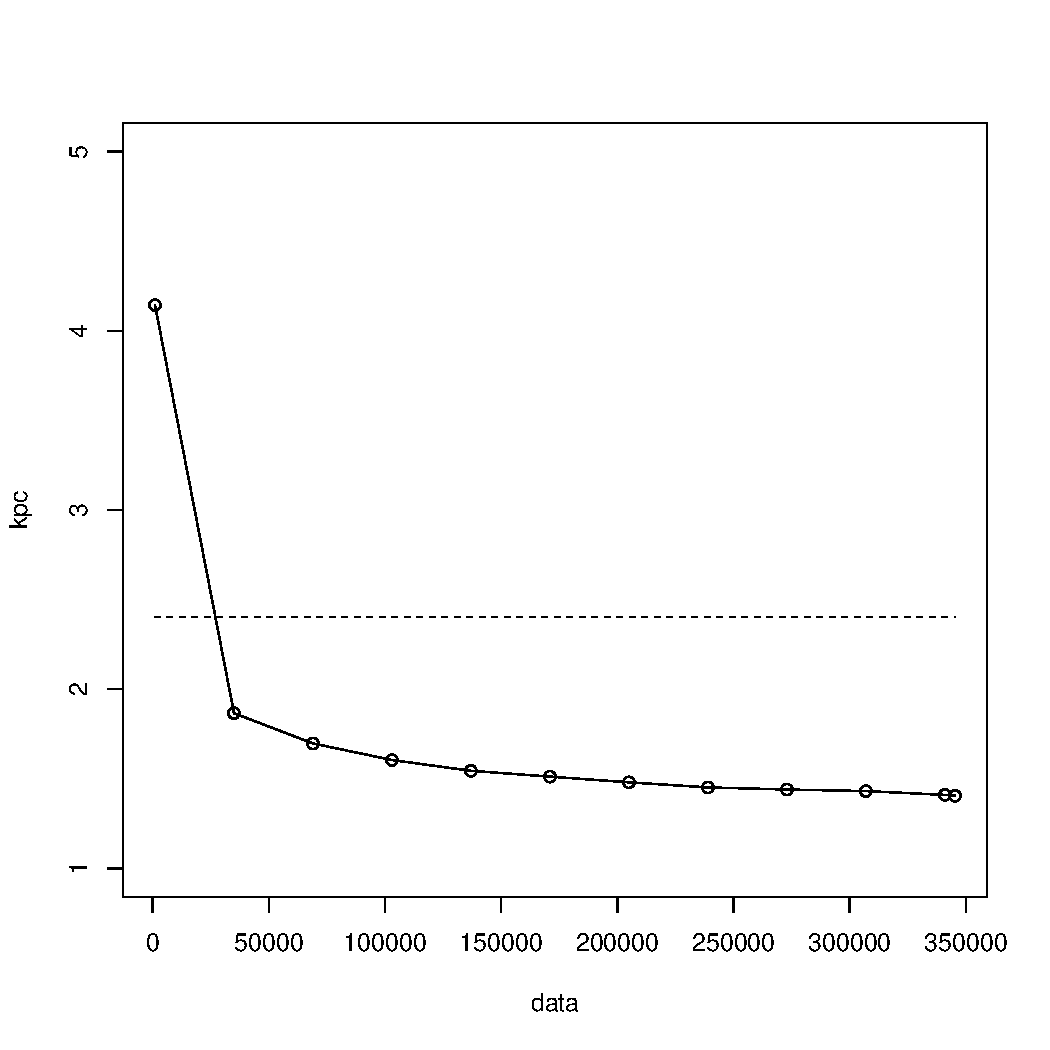
\includegraphics[width=2.5in]{finnish_kpc_figure.pdf}
\end{center}
\caption{The effect of the amount of training data (horizontal axis)
  on the KPC ratio (vertical axis) of the Finnish predictive text
  entry system. The dashed line shows the KPC for
  multitap. The minimal KPC ratio is 1.3818.}\label{fi-kpc-graph}
\end{figure}

We compared our system to another published Finnish text-entry system
by~\cite{silfverberg/2011/cla}, which is based on a morphological
analyzer and a colloquial dictionary. They do not evaluate their
system using the KPC ratio, but we were able to obtain their test
results and according to our experiments they achieve a KPC ratio of
$1.6120$. This means that our system achieves a 14.3\% decrease in KPC
compared with the dictionary-based system using the same training
materials and test data, but without using the morphological
analyzer. \footnote{When examining the test data used by
  \cite{silfverberg/2011/cla}, we discovered, that the latter half of
  the data consisted of a uniquified word list, which affected their
  results negatively. We have computed the KPC ratio for both our own
  system and the system of \cite{silfverberg/2011/cla} using only the
  $6663$ first words in the test data.}

\begin{table}
\begin{center}
\caption{KPC for Finnish Multitap and for using different components of
  our system. The third column shows the improvement over
  multitap.}\label{Finnish-kpc-table}
\begin{tabular}{lcr}
\hline
Method ~~~~& ~~~~KPC~~~~ &~~~~Improvement (\%)\\
\hline
Multitap                                       &2.4018 & 0.0~~~~~~~~~~\\
Letter n-grams                                 &1.7368 & 27.7~~~~~~~~~~\\
Letter n-grams and morph sequence model        &1.3825 & 43.4~~~~~~~~~~\\
Letter n-grams, morph sequence model and rules &1.3818 & 43.5~~~~~~~~~~\\
\hline
\end{tabular}
\end{center}
\end{table}

In practice, ten suggestions for an input sequence is quite a lot. Few
users are likely to scroll through ten suggestions especially if there
are many non-words in the suggestion list. Therefore we also computed
the KPC ratio for the entire training data as a function of the number
of suggestions given by the system. The results are shown in
Figure~\ref{fi-kpc-suggestions}.

\begin{table}\label{fi-kpc-suggestions}
\caption{The effect of the number of suggestions on the KPC ratio of the Finnish text entry system using all of the training data.}
\begin{center}
\begin{tabular}{lcccccccccc}
\hline
\# of Sugg.~~&  1 & 2 & 3 & 4 & 5 & 6 & 7 & 8 & 9 & 10\\
\hline
KPC & 2.1428 & 1.7431 & 1.6036 & 1.5251 & 1.4845 & 1.4355 & 1.4065 & 1.3920 & 1.3846 & 1.3818\\
\hline
\end{tabular}
\end{center}
\end{table}

Finally we wanted to compare our system to some commercially available
text entry systems. To accomplish this, we took a list of thirty words
chosen at random from the training data, entered the words into three
commercially available mobile phones and computed the KPC ratio. We
also tested our own system using the words. Since the text entry
system of the mobile phones did not give ten suggestions, we computed
results only on the three first guesses given by each system. The
results are shown in Table~\ref{mobile-phone-kpc}.

\begin{table}
\caption{The KPC ratio for the text entry of two commercial phones and
  our system using a $30$ word random sample from our test data. Only
  the three first suggestions were considered for each system.}\label{mobile-phone-kpc}
\begin{center}
\begin{tabular}{lc}
\hline
System & KPC\\
\hline
Nokia 2600       & 1.9576\\
Samsung SGH M310 & 1.9576\\
Nokia C7         & 2.1557\\
Our system       & 1.3350\\
\hline
\end{tabular}
\end{center}
\end{table}

\subsection{Results for Turkish}

For Turkish, we trained one system using the entire $20$ million word
training corpus, which was presented in section~\ref{data}. We compare
our results against the predictive text entry system
by~\cite{Tantug:2010}.

For the multitap method, our figure for the KPC ratio $2.4386$ differs
slightly from the figure $2.2014$ given by~\cite{Tantug:2010}. There
is some concern that the figure $2.2014$ is erroneously computed by
computing the length of words in bytes rather than in utf-8
characters. If we substitute the length of words in utf-8 characters
by the incorrect length. We arrive at a figure $2.20914$, which is
very close to $2.2014$. Because of this inconsistency, it is possible
that our results are not entirely comparable to the results
of~\cite{Tantug:2010}. The improvement in KPC ratio given for the method
by~\cite{Tantug:2010} is computed using our figure for the KPC ratio
of the multitap method. The improvement given by~\cite{Tantug:2010} is
$35\%$.

\begin{table}
\caption{KPC for Turkish using different input methods. The third
  column shows the improvement over the multitap method.}\label{Turkish-kpc-table}
\begin{center}
\begin{tabular}{lcr}
\hline
Method~~~~& ~~~~KPC~~~~ & ~~~~Improvement (\%)\\
\hline
Multitap                          &  2.4386 &0.0~~~~~~~~~~\\
Letter n-grams~\cite{Tantug:2010} &  1.4382 &41.0~~~~~~~~~~\\
Our method                        &  1.1768 &51.7~~~~~~~~~~\\
\hline
\end{tabular}
\end{center}
\end{table}

\section{Discussion}\label{discussion}

For Finnish our system achieves a substantial $14.3\%$ drop in KPC
ratio compared with the other system which utilizes a morphological
analyzer. In their Finnish text entry
system~\cite{silfverberg/2011/cla} give only $3$ suggestions. Looking
at Table~\ref{fi-kpc-suggestions} we see that the KPC ratio for our
system is $1.6036$, when only considering the three first suggestions,
which is still lower than the KPC ratio $1.6120$, which their system
achieves. Considering, that except the phonological constraints, we
use only language independent components, this is remarkable.

The phonological constraints seem to be having very little effect, as
can be seen in Table~\ref{Finnish-kpc-table}. The decrease in KPC when
using the phonological constraints is only about $0.1\%$. This may be
a result of the unsupervised segmentation, which does not always
succeed in finding the correct morpheme boundaries and therefore may
prevent the rules from being triggered.

As Figure~\ref{mobile-phone-kpc} shows, our system outperforms three
commercially available mobile phones on a thirty word test set chosen
at random from our test data. This shows that our approach has great
practical potential.

As can be seen in Table~\ref{Turkish-kpc-table} our method achieves an
additional $10\%$ point reduction in KPC for Turkish compared to the
system in~\cite{Tantug:2010}. Our KPC ratio $1.1768$ needs to be
related to the fact that our method can never achieve a KPC ratio
lower than $1$, since every letter in a word needs to be typed. We
achieve a $51.7\%$ reduction in KPC for the Turkish test data compared
to the multitap method. A fast computation reveals that the maximal
possible reduction is only $59.0\%$, which demonstrates that our
system is nearly optimal on the Turkish data.

\section{Conclusions and future work}\label{conclusion}

We have demonstrated a highly efficient predictive text entry model,
which can be constructed using unsupervised methods. Additionally
linguistic rules can be added to improve the performance of the
system.

There are several interesting future research directions. In order to
reduce the KPC ratio to $< 1$, the system should be able to predict
morphs before they are completely typed. We should also consider
adding a model, which extends over word boundaries.

It would be interesting to examine the effect of the segmentation of
the training corpus on the function of the phonological rules. A
linguistically soundly segmented training corpus would probably allow
the rules to act more often and thus improve the KPC ratio.

\section{Acknowledgments}
\ldots\\
\ldots\\
\ldots


\bibliographystyle{splncs03}
\bibliography{cicling2011.bib}
\end{document}
